\documentclass[aspectratio=169]{beamer}

\usepackage{ccicons}
\usepackage{fontspec}
\usepackage{listings}
\usepackage{tikz}
\usepackage{svg}

\definecolor{uclablue}{RGB}{39,116,174}
\definecolor{uclagold}{RGB}{255,179,0}

\definecolor{ubcorange}{RGB}{158, 66, 37}

\definecolor{cugold}{RGB}{207, 184, 124}
\definecolor{cudarkgray}{RGB}{86, 90, 92}

\definecolor{solarizedred}{RGB}{220, 50, 47}
\definecolor{solarizedblue}{RGB}{38, 139, 210}
\definecolor{solarizedgreen}{RGB}{133, 153, 0}
\definecolor{solarizedpurple}{RGB}{108, 113, 196}
\definecolor{solarizedmagenta}{RGB}{211, 54, 130}

\definecolor{pantone655}{RGB}{0, 42, 92}
\definecolor{pantone7453}{RGB}{123, 164, 217}
\definecolor{pantone633}{RGB}{0, 139, 176}
\definecolor{pantone7492}{RGB}{218, 229, 205}

\colorlet{primarycolor}{pantone655}
\colorlet{secondarycolor}{pantone7453}


\usetikzlibrary{
  arrows,
  arrows.meta,
  automata,
  backgrounds,
  calc,
  chains,
  decorations.pathreplacing,
  fit,
  intersections,
  matrix,
  overlay-beamer-styles,
  positioning,
  shapes,
  shapes.multipart,
  tikzmark,
}
\usetikzmarklibrary{listings}

\hypersetup{
  colorlinks=true,
  urlcolor=cudarkgray,
}

\setbeamercolor{frametitle}{fg=primarycolor}
\setbeamercolor{structure}{fg=primarycolor}
\setbeamercolor{enumerate item}{fg=black}
\setbeamercolor{itemize item}{fg=black}
\setbeamercolor{itemize subitem}{fg=black}

\setbeamersize{text margin left=26.6mm}
\addtolength{\headsep}{2mm}

\setbeamertemplate{navigation symbols}{}
\setbeamertemplate{headline}{}
\setbeamertemplate{footline}{}
\setbeamertemplate{itemize item}{\color{black}}
\setbeamertemplate{itemize items}[circle]

\setbeamertemplate{footline}{
  \begin{tikzpicture}[remember picture,
                      overlay,
                      shift={(current page.south west)}]
    \node [black!50, inner sep=2mm, anchor=south east]
          at (current page.south east) {\footnotesize \insertframenumber};
  \end{tikzpicture}
}

\setsansfont{Inter}[Scale=MatchLowercase]
\setmonofont{Hack}[Scale=MatchLowercase]

\makeatletter
\newcommand\version[1]{\renewcommand\@version{#1}}
\newcommand\@version{}
\def\insertversion{\@version}

\newcommand\lecturenumber[1]{\renewcommand\@lecturenumber{#1}}
\newcommand\@lecturenumber{}
\def\insertlecturenumber{\@lecturenumber}
\makeatother

\setbeamertemplate{title page}
{
  \begin{tikzpicture}[remember picture,
                      overlay,
                      shift={(current page.south west)},
                      background rectangle/.style={fill=pantone655},
                      show background rectangle]
    \node [anchor=west, align=left, inner sep=0, text=white]
          (lecturenumber) at (\paperwidth / 6, \paperheight * 3 / 4)
          {\Large Lecture \insertlecturenumber};
    \node [inner sep=0, align=left, text=white, node distance=0,
          above left=of lecturenumber, anchor=south west, yshift=2mm]
          {\Large ECE 344: Operating Systems};
    \node (title) [inner sep=0, anchor=west, align=left, text=white,
                   text width=30em]
          at (\paperwidth / 6, \paperheight / 2)
          {{\bfseries \Huge \inserttitle{}}};
    \node [inner sep=0, align=right, text=white, node distance=0,
          below right=of title, anchor=north east, yshift=-1mm]
          {{\footnotesize \ttfamily \insertversion}};
    \node [inner sep=0, text=white, align=left, anchor=west]
          (author) at (\paperwidth / 6, \paperheight / 4)
          {\insertauthor};
    \node [text=white, inner sep=0, align=left, node distance=0,
           below left=of author, anchor=north west, yshift=-2mm]
          {\insertdate};
    \node [align=right, anchor=south east, inner sep=2mm, text=white]
          (license) at (\paperwidth, 0)
          {\footnotesize This  work is licensed under a
           \href{http://creativecommons.org/licenses/by-sa/4.0/}
                {\color{pantone7453} Creative Commons Attribution-ShareAlike 4.0
                 International License}};
    \node [text=white, inner sep=0, align=right, node distance=0,
           above right=of license, anchor=south east, xshift=-2mm]
          {\Large \ccbysa};
  \end{tikzpicture}
}

\tikzset{
  >=Straight Barb[],
  shorten >=1pt,
  initial text=,
}

\lstset{
  basicstyle=\footnotesize\ttfamily,
  language=C,
  escapechar=@,
  commentstyle=\color{black!50},
}


\lecturenumber{25}
\title{More Memory Allocation}
\version{1.0.0}
\author{Jon Eyolfson}
\date{November 15/16, 2022}

\begin{document}
  \begin{frame}[plain, noframenumbering]
    \titlepage
  \end{frame}

  \begin{frame}
    \frametitle{The Buddy Allocator Restricts the Problem}

    Typically allocation requests are of size $\mathsf{2^n}$

    \hspace{2em} e.g. 2, 4, 8, 16, 32, ..., 4096, ...

    \vspace{2em}

    Restrict allocations to be powers of 2 to enable a more efficient
    implementation

    \hspace{2em} Split blocks into 2 until you can handle the request

    \vspace{2em}

    We want to be able to do fast searching and merging
  \end{frame}

  \begin{frame}
    \frametitle{You Can Implement the Buddy Allocator Using Multiple Lists}
    

    We restrict the requests to be $\mathsf{2^k, 0 \leq k \leq N}$ (round up if
    needed)

    \vspace{2em}

    Our implementation would use $\mathsf{N+1}$ free lists of blocks for each
    size

    \hspace{2em}

    For a request of size $\mathsf{2^k}$, we search the free list until we find
    a big enough block

    \hspace{2em} Search $\mathsf{k, k+1, k+2, ...}$ until we find one

    \hspace{4em} Recursively divide the block if needed until it's the correct
                 size

    \hspace{6em} Insert “buddy” blocks into free lists

    \vspace{2em}

    For deallocations, we coalesce the buddy blocks back together

    \hspace{2em} Recursively coalesce the blocks if needed
  \end{frame}

  \begin{frame}{Using the Buddy Allocator (1)}

    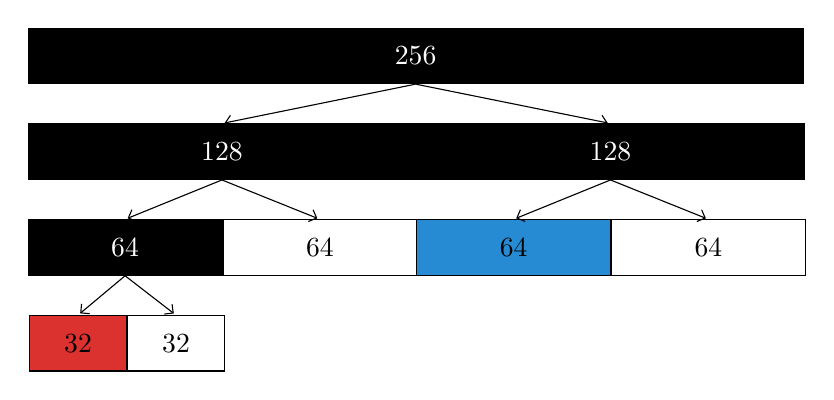
\begin{tikzpicture}[node distance=5mm and 0mm]
            
        \node[draw,rectangle,minimum width=280,minimum height=20,fill=black,text=white]    (a00)        {256};
        \node[draw,rectangle,minimum width=140,minimum height=20,fill=black,text=white,xshift=-70]    (a10) [below=of a00]       {128};
        \node[draw,rectangle,minimum width=140,minimum height=20,fill=black,text=white]    (a11) [right=of a10]       {128};
        \node[draw,rectangle,minimum width=70,minimum height=20,fill=black,text=white,xshift=-35]    (a20) [below=of a10]       {64};
        \node[draw,rectangle,minimum width=70,minimum height=20]    (a21) [right=of a20]       {64};
        \node[draw,rectangle,minimum width=70,minimum height=20,fill=solarizedblue,xshift=-35]    (a22) [below=of a11]       {64};
        \node[draw,rectangle,minimum width=70,minimum height=20]    (a23) [right=of a22]       {64};
        \node[draw,rectangle,minimum width=35,minimum height=20,fill=solarizedred,xshift=-17]    (a30) [below=of a20]       {32};
        \node[draw,rectangle,minimum width=35,minimum height=20]    (a31) [right=of a30]       {32};

        \draw[->] (a00.south) -- (a10.north);
        \draw[->] (a00.south) -- (a11.north);
        \draw[->] (a10.south) -- (a20.north);
        \draw[->] (a10.south) -- (a21.north);
        \draw[->] (a11.south) -- (a22.north);
        \draw[->] (a11.south) -- (a23.north);
        \draw[->] (a20.south) -- (a30.north);
        \draw[->] (a20.south) -- (a31.north);

    \end{tikzpicture}

    \vspace{2em}

    Where do we allocate a request of size 28?
  \end{frame}

  \begin{frame}{Using the Buddy Allocator (2)}

    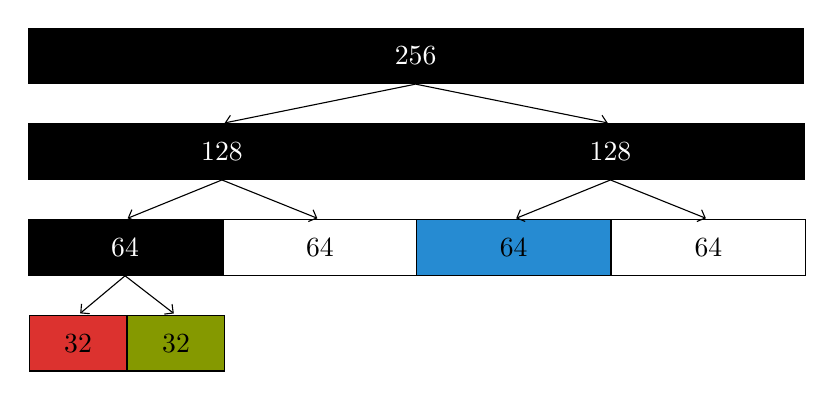
\begin{tikzpicture}[node distance=5mm and 0mm]
            
        \node[draw,rectangle,minimum width=280,minimum height=20,fill=black,text=white]    (a00)        {256};
        \node[draw,rectangle,minimum width=140,minimum height=20,fill=black,text=white,xshift=-70]    (a10) [below=of a00]       {128};
        \node[draw,rectangle,minimum width=140,minimum height=20,fill=black,text=white]    (a11) [right=of a10]       {128};
        \node[draw,rectangle,minimum width=70,minimum height=20,fill=black,text=white,xshift=-35]    (a20) [below=of a10]       {64};
        \node[draw,rectangle,minimum width=70,minimum height=20]    (a21) [right=of a20]       {64};
        \node[draw,rectangle,minimum width=70,minimum height=20,fill=solarizedblue,xshift=-35]    (a22) [below=of a11]       {64};
        \node[draw,rectangle,minimum width=70,minimum height=20]    (a23) [right=of a22]       {64};
        \node[draw,rectangle,minimum width=35,minimum height=20,fill=solarizedred,xshift=-17]    (a30) [below=of a20]       {32};
        \node[draw,rectangle,minimum width=35,minimum height=20,fill=solarizedgreen]    (a31) [right=of a30]       {32};

        \draw[->] (a00.south) -- (a10.north);
        \draw[->] (a00.south) -- (a11.north);
        \draw[->] (a10.south) -- (a20.north);
        \draw[->] (a10.south) -- (a21.north);
        \draw[->] (a11.south) -- (a22.north);
        \draw[->] (a11.south) -- (a23.north);
        \draw[->] (a20.south) -- (a30.north);
        \draw[->] (a20.south) -- (a31.north);

    \end{tikzpicture}

    \vspace{2em}

    Where do we allocate a request of size 32?
  \end{frame}

  \begin{frame}{Using the Buddy Allocator (3)}

    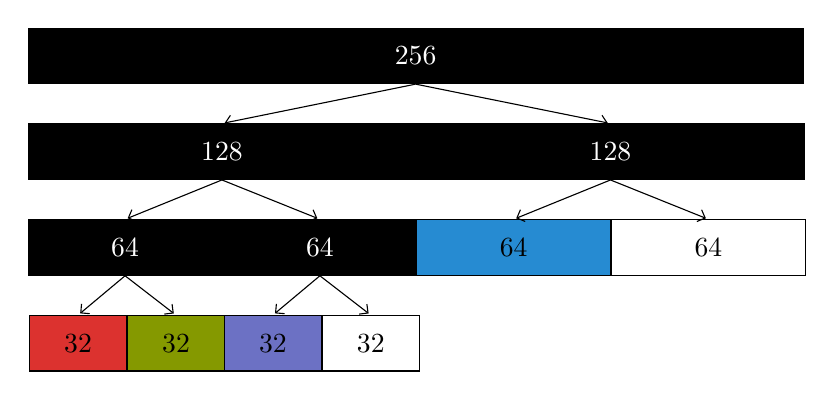
\begin{tikzpicture}[node distance=5mm and 0mm]
            
        \node[draw,rectangle,minimum width=280,minimum height=20,fill=black,text=white]    (a00)        {256};
        \node[draw,rectangle,minimum width=140,minimum height=20,fill=black,text=white,xshift=-70]    (a10) [below=of a00]       {128};
        \node[draw,rectangle,minimum width=140,minimum height=20,fill=black,text=white]    (a11) [right=of a10]       {128};
        \node[draw,rectangle,minimum width=70,minimum height=20,fill=black,text=white,xshift=-35]    (a20) [below=of a10]       {64};
        \node[draw,rectangle,minimum width=70,minimum height=20,fill=black,text=white]    (a21) [right=of a20]       {64};
        \node[draw,rectangle,minimum width=70,minimum height=20,fill=solarizedblue,xshift=-35]    (a22) [below=of a11]       {64};
        \node[draw,rectangle,minimum width=70,minimum height=20]    (a23) [right=of a22]       {64};
        \node[draw,rectangle,minimum width=35,minimum height=20,fill=solarizedred,xshift=-17]    (a30) [below=of a20]       {32};
        \node[draw,rectangle,minimum width=35,minimum height=20,fill=solarizedgreen]    (a31) [right=of a30]  {32};
        \node[draw,rectangle,minimum width=35,minimum height=20,fill=solarizedpurple,xshift=-17]    (a32) [below=of a21]       {32};
        \node[draw,rectangle,minimum width=35,minimum height=20,]    (a33) [right=of a32]       {32};

        \draw[->] (a00.south) -- (a10.north);
        \draw[->] (a00.south) -- (a11.north);
        \draw[->] (a10.south) -- (a20.north);
        \draw[->] (a10.south) -- (a21.north);
        \draw[->] (a11.south) -- (a22.north);
        \draw[->] (a11.south) -- (a23.north);
        \draw[->] (a20.south) -- (a30.north);
        \draw[->] (a20.south) -- (a31.north);
        \draw[->] (a21.south) -- (a32.north);
        \draw[->] (a21.south) -- (a33.north);

    \end{tikzpicture}

    \vspace{2em}

    What happens when the we free the size 64 block?
\end{frame}


  \begin{frame}{Using the Buddy Allocator (4)}

    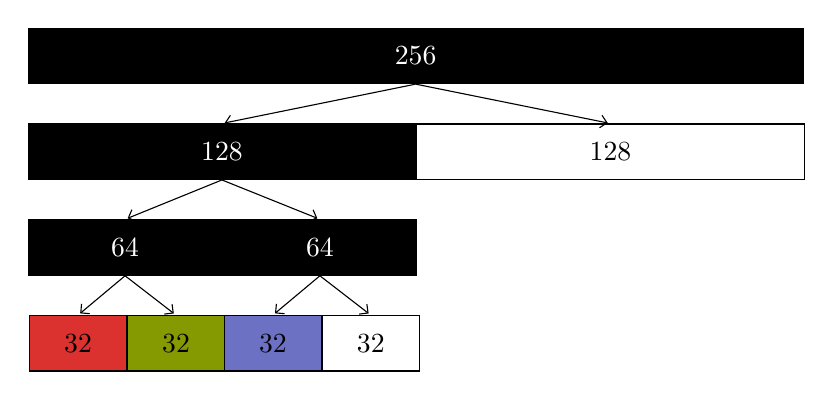
\begin{tikzpicture}[node distance=5mm and 0mm]
            
        \node[draw,rectangle,minimum width=280,minimum height=20,fill=black,text=white]    (a00)        {256};
        \node[draw,rectangle,minimum width=140,minimum height=20,fill=black,text=white,xshift=-70]    (a10) [below=of a00]       {128};
        \node[draw,rectangle,minimum width=140,minimum height=20]    (a11) [right=of a10]       {128};
        \node[draw,rectangle,minimum width=70,minimum height=20,fill=black,text=white,xshift=-35]    (a20) [below=of a10]       {64};
        \node[draw,rectangle,minimum width=70,minimum height=20,fill=black,text=white]    (a21) [right=of a20]       {64};
        \node[draw,rectangle,minimum width=35,minimum height=20,fill=solarizedred,xshift=-17]    (a30) [below=of a20]       {32};
        \node[draw,rectangle,minimum width=35,minimum height=20,fill=solarizedgreen]    (a31) [right=of a30]  {32};
        \node[draw,rectangle,minimum width=35,minimum height=20,fill=solarizedpurple,xshift=-17]    (a32) [below=of a21]       {32};
        \node[draw,rectangle,minimum width=35,minimum height=20,]    (a33) [right=of a32]       {32};

        \draw[->] (a00.south) -- (a10.north);
        \draw[->] (a00.south) -- (a11.north);
        \draw[->] (a10.south) -- (a20.north);
        \draw[->] (a10.south) -- (a21.north);
        \draw[->] (a20.south) -- (a30.north);
        \draw[->] (a20.south) -- (a31.north);
        \draw[->] (a21.south) -- (a32.north);
        \draw[->] (a21.south) -- (a33.north);

    \end{tikzpicture}

  \end{frame}

  \begin{frame}
    \frametitle{Buddy Allocators are Used in Linux}


    Advantages

    \hspace{2em} Fast and simple compared to general dynamic memory allocation

    \hspace{2em} Avoids external fragmentation by keeping free physical pages contiguous

    \vspace{2em}

    Disadvantages

    \hspace{2em} There's always internal fragmentation

    \hspace{4em} We always round up the allocation size if it's not a power of 2
  \end{frame}

  \begin{frame}{Slab Allocators Take Advantage of Fixed Size Allocations}

  Allocate objects of same size from a dedicated pool

  \hspace{2em} All structures of the same type are the same size

  \vspace{2em}

  Every object type has it's own pool with blocks of the correct size

    \hspace{2em} This prevents internal fragmentation
  \end{frame}

  \begin{frame}
    \frametitle{Slab is a Cache of ``Slots''}

    Each allocation size has a corresponding slab of slots (one slot holds one
    allocation)

    \vspace{2em}

    Instead of a linked list, we can use a bitmap (there's a mapping between
    bit and slot)

    \hspace{2em} For allocations we set the bit and return the slot

    \hspace{2em} For deallocations we just clear the bit

    \vspace{2em}

    The slab an be implemented on top of the buddy allocator
  \end{frame}

  \begin{frame}{Each Slab Can Be Allocated using the Buddy Allocator}
    
    Consider two object sizes: A and B

    \vspace{2em}
    
    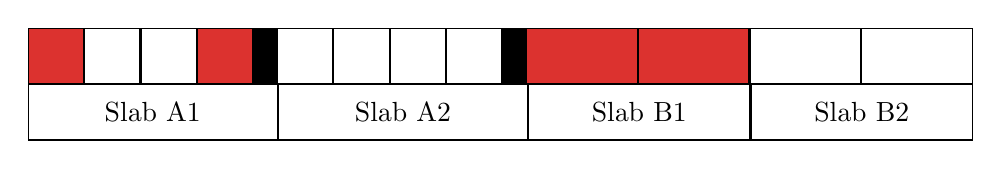
\begin{tikzpicture}[node distance=0mm and 0mm]

        \node[draw,rectangle,minimum width=20,minimum height=20,fill=solarizedred]    (a0)        {};
        \node[draw,rectangle,minimum width=20,minimum height=20]    (a1)     [right=of a0]   {};
        \node[draw,rectangle,minimum width=20,minimum height=20]    (a2)     [right=of a1]   {};
        \node[draw,rectangle,minimum width=20,minimum height=20,fill=solarizedred]    (a3)     [right=of a2]   {};
        \node[draw,rectangle,minimum width=8,minimum height=20,fill=black]    (a4)     [right=of a3]   {};

        \node[draw,rectangle,minimum width=20,minimum height=20]    (a5)     [right=of a4]   {};
        \node[draw,rectangle,minimum width=20,minimum height=20]    (a6)     [right=of a5]   {};
        \node[draw,rectangle,minimum width=20,minimum height=20]    (a7)     [right=of a6]   {};
        \node[draw,rectangle,minimum width=20,minimum height=20]    (a8)     [right=of a7]   {};
        \node[draw,rectangle,minimum width=8,minimum height=20,fill=black]    (a9)     [right=of a8]   {};


        \node[draw,rectangle,minimum width=40,minimum height=20,fill=solarizedred]    (b1)     [right=of a9]   {};
        \node[draw,rectangle,minimum width=40,minimum height=20,fill=solarizedred]    (b2)     [right=of b1]   {};

        \node[draw,rectangle,minimum width=40,minimum height=20]    (b3)     [right=of b2]   {};
        \node[draw,rectangle,minimum width=40,minimum height=20]    (b4)     [right=of b3]   {};

        \node[draw,rectangle,minimum width=90,minimum height=20,xshift=35]    (s0)    [below=of a0]   {Slab A1};
        \node[draw,rectangle,minimum width=90,minimum height=20]    (s1)    [right=of s0]   {Slab A2};
        \node[draw,rectangle,minimum width=80,minimum height=20]    (s2)    [right=of s1]   {Slab B1};
        \node[draw,rectangle,minimum width=80,minimum height=20]    (s3)    [right=of s2]   {Slab B2};

    \end{tikzpicture}

    \vspace{2em}

    We can reduce internal fragmentation if Slabs are located
    adjacently

    \hspace{2em} In this example A has internal fragmentation (dark box)
  \end{frame}

  \begin{frame}
    \frametitle{Even More Memory Allocations}

    The kernel restricts the problem for better memory allocation
    implementations

    \begin{itemize}
      \item Buddy allocator is a real world restricted implementation
      \item Slab allocator takes advantage of fixed sized objects to reduce
            fragmentation
    \end{itemize}
  \end{frame}
\end{document}
